\documentclass{article}
\usepackage{graphicx} % new way of doing eps files
\usepackage{listings} % nice code layout
\usepackage[usenames]{color} % color
\definecolor{listinggray}{gray}{0.9}
\definecolor{graphgray}{gray}{0.7}
\definecolor{ans}{rgb}{1,0,0}
\definecolor{blue}{rgb}{0,0,1}
% \Verilog{title}{label}{file}
\graphicspath{ {H:/ELC3338/Team8/CompOrg_Spring2018_S1_Team8/images/} }
\newcommand{\Verilog}[3]{
  \lstset{language=Verilog}
  \lstset{backgroundcolor=\color{listinggray},rulecolor=\color{blue}}
  \lstset{linewidth=\textwidth}
  \lstset{commentstyle=\textit, stringstyle=\upshape,showspaces=false}
  \lstset{frame=tb}
  \lstinputlisting[caption={#1},label={#2}]{#3}
}


\author{Matthew Carrano and Breana Leal}
\title{Lab 3}

\begin{document}
\maketitle

\section{Introduction}
The goal of this lab is to complete the Decode stage and connect the stage following the Fetch stage.

\section{Interface}
The input for iDecode is currently the hard written write\_data instructions given by the expected results table. Once established, the input is the outputted instruction from the iFetch stage. The instruction is used internally for the sign extender, mux, regfile, and control modules. The outputs for iDecode are the control module outputs expect those that are maintained internally (RegWrite and Reg2Loc) and a 64 bit sign-extended instruction.

The datapath module is provided as a link between the two stages. Based on Figure 6.1, there is one single wire connection from the iFetch to the iDecode. The link is the final instruction from the iFetch to serve as the iDecode input. The datapath outputs match the same as mentioned in the iDecode module.

\section{Design}
iDecode is one unit with five internal modules. The modules are instr\_parse, mux, sign\_extender, control, and regfile. The decode uses a 32 bit instruction to work internally to output a 64 bit output from the sign -extender, outputs read\_data1 and read\_data2 from the regfile (has a fed input from the mux output), and various control outputs.

The datapath testbench module engages the iDecode and iFetch modules to link the two. Again, the Decode stage will process the outputted instruction from the Fetch stage.
 
\section{Implementation}
The iDecode module is implemented by instantiating the five internal modules. The inputs are clk, read\_clk, write\_clk, and a 32 bit instr. The nine outputs are uncondbranch, branch, mem\_read, mem\_to\_reg, alu\_op, mem\_write,  alu\_src, ext\_adder, and alu\_con\_instru. The first seven of the outputs come from the control. There are seven wires that are internally used to link. reg\_write, reg2\_loc, read\_reg2, opcode, rm , rn, and rd. reg\_write and reg2\_loc are maintained internally, feeding into the mux and regfile. The remaining wires are for the instr\_parse to appropriately breakdown the provided instruction for the mux.

Essentially, the input instruction's rm and rd are inputs for the mux. Based on the reg2\_loc mux control the decided output, read\_reg2, is fed into the regfile. Additionally, the instruction is fed into the sign-extender where the destination address is extended to 64 bits. Control has the same functionally in terms of inputs and outputs but its reg\_write serves as a component for the regfile. 

The elaborated schematic Figure 1 , further in the report, provides the overview of the code implementation for the iDecode. 

	The datapath will serve as the testbench for the entire ARM-Lab project. For this lab, it houses the first two stages. The iFetch flowing into the iDecode stage and the iDecode stage ending with its open outputs for future stages.

\Verilog{Verilog code for implementing the mux module.}{code:mux}{../code/0_common/mux.v}

\Verilog{Verilog code for implementing the instr\_parse module.}{code:mux}{../code/2_decode/instr_parse.v}

\Verilog{Verilog code for implementing the sign\_extender module.}{code:mux}{../code/2_decode/sign_extender.v}

\Verilog{Verilog code for implementing the control module.}{code:mux}{../code/2_decode/control.v}

\Verilog{Verilog code for implementing the regfile module.}{code:mux}{../code/2_decode/regfile.v}

\Verilog{Verilog code for implementing the iDecode module.}{code:mux}{../code/2_decode/iDecode.v}

\begin{figure}[h]	
	\caption{Elaborated Schematic for iDecode.}
	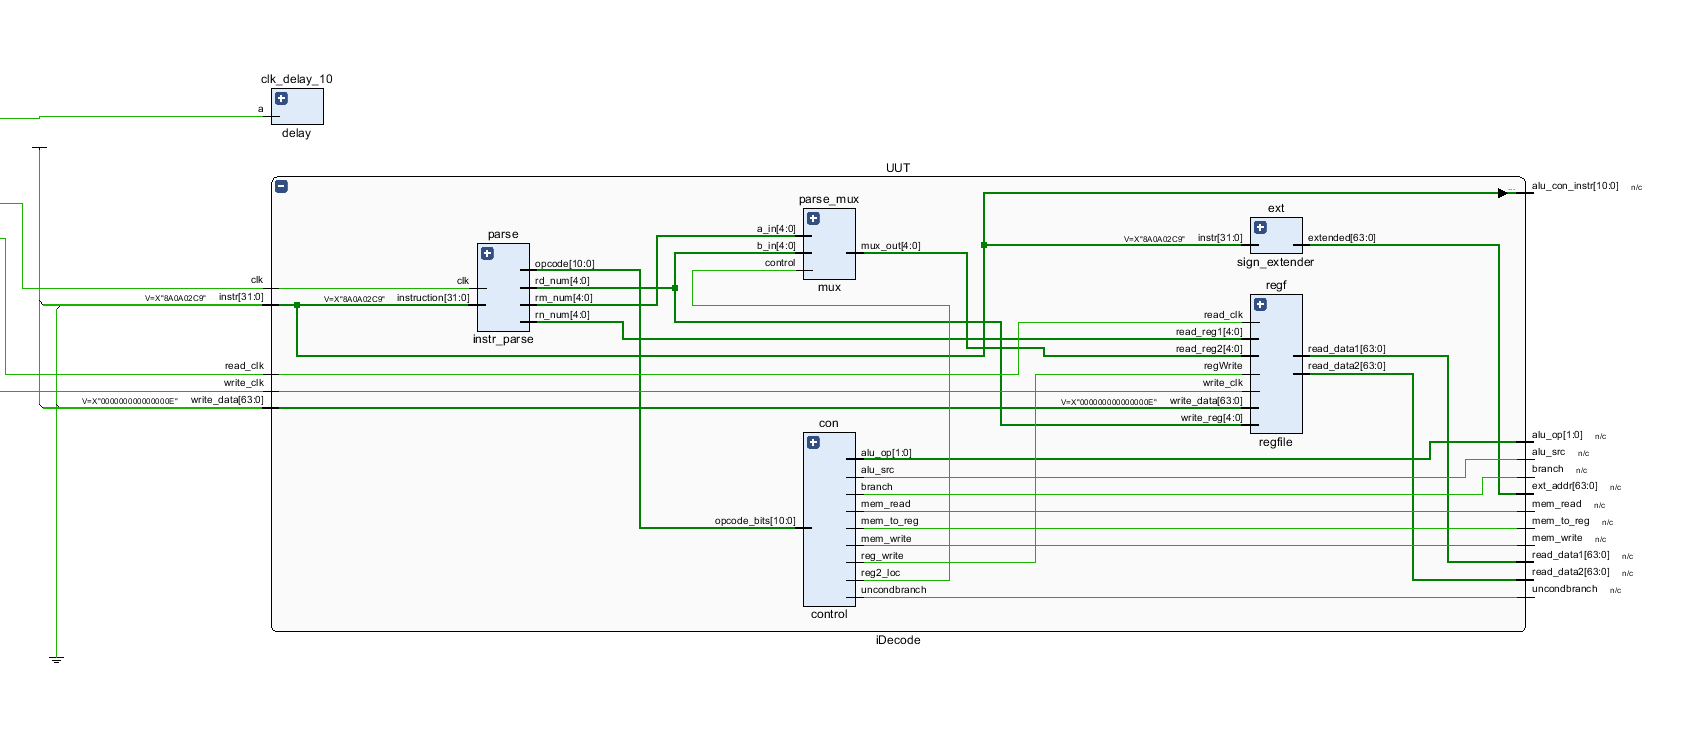
\includegraphics[width=\textwidth]{elaborated_decode}
	\label{fig:fetchtest}
\end{figure}


\section{Test Bench Design}
A test bench was made for each module. The testbench for the iDecode has wires for its external pieces and its outputs, clk, read\_clk, write\_clk, and remaining control outputs not internally maintained. To adjust for timing with the modules, there are a series of ten clk delays. Each delay follows the format of clk\_delay\_1 or the corresponding instruction number (1-10). The delays establish the ARM's synchronization.
The ten cases are the hard written machine code in hex (instr) and write\_data provided by the expected results table.

\Verilog{Verilog code for testing the Decode stage.}{code:instrtest}{../code/2_decode/iDecode_test.v}

Next, datapath is created as a final destination testbench to oversee all of the ARM's actions and designated debugging area. Its inputs and ouputs remain as mentioned earlier and again bridge the first two ARM stages.
 
\Verilog{Verilog code for testing the datapath testbench.}{code:mux}{../code/2_decode/datapath.v} 

\section{Simulation}
The timing diagrams in Figure 3 and 4 verify that both modules work as detailed in the above section. One way to easily verify functionality for the iDecode is to compare the outputs to the data of Figure 2, the Expected Results Table. 

\begin{figure}[h]	
	\caption{Expected Results Table.}
	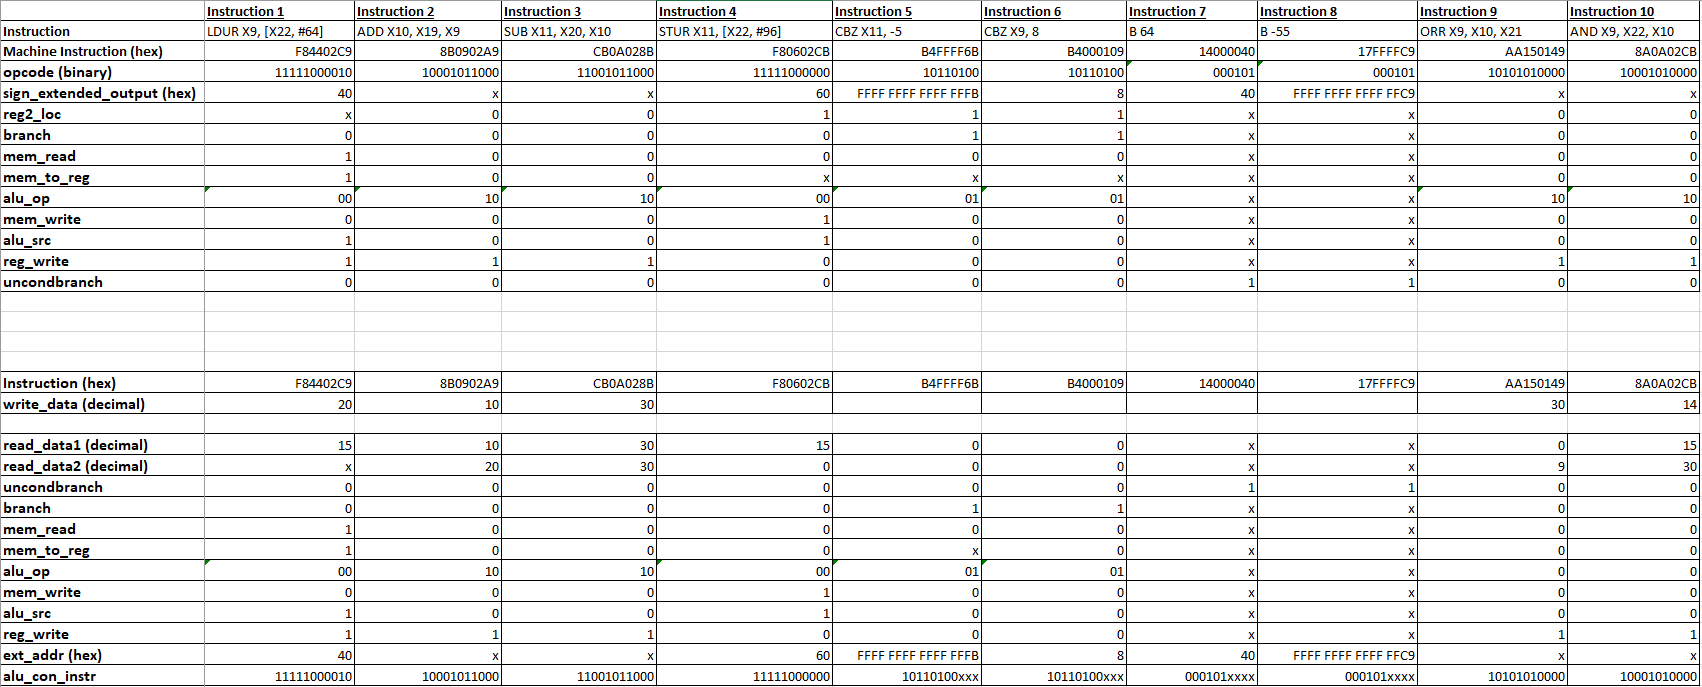
\includegraphics[width=\textwidth]{Expected_results_table}
	\label{fig:fetchtest}
\end{figure}

\begin{figure}[h]	
	\caption{Timing diagram for iDecode module test.}
	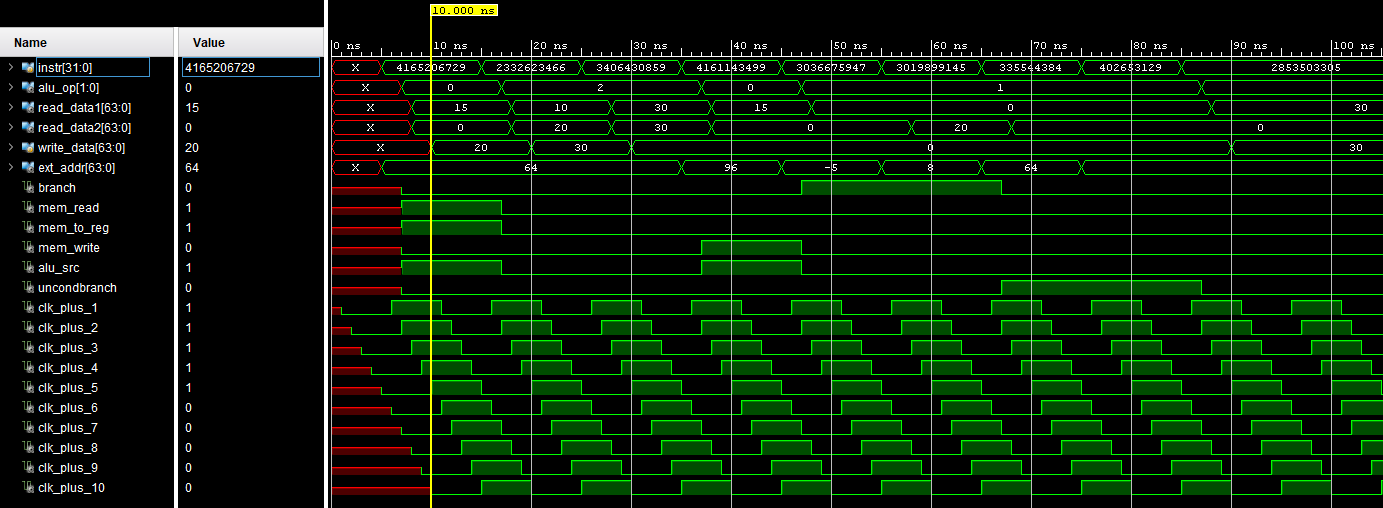
\includegraphics[width=\textwidth]{iDecode_Sim}
	\label{fig:instrmemtest}
\end{figure}

\begin{figure}[h]	
	\caption{Timing diagram for datapath module test.}
	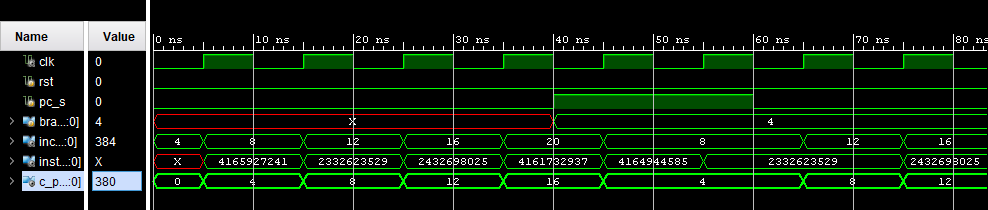
\includegraphics[width=\textwidth]{fetch_sim}
	\label{fig:fetchtest}
\end{figure}


\section{Conclusions}
The iDecode module and datapath testbench were successfully established. iDecode is our second stage that uses the instruction for sign extending, controlling, and processing in the regfile using the mux. Its outputs are those from the control not internally maintained. Its input is the iFetch's instructional output. The iFetch is linked with the iDecode stage with the datapath testbench. The testbench demonstrates the ARM's increments fetched at proper times.
 

\end{document} 